\documentclass[10pt]{article}
%%%%%%%%%%%%%%%%%%%%%%%%%%%%%%%%%%%%%%%%
\usepackage{amsmath}
\usepackage{verbatim}
\usepackage[usenames,dvipsnames]{color}
\usepackage{ulem}
\usepackage{setspace}
\usepackage{lscape}
\usepackage{longtable}
\usepackage[top=1.25in,bottom=1.5in,left=1in,right=1.5in,landscape]{geometry}
\usepackage{graphicx}
\usepackage{epstopdf}
\usepackage[usenames,dvipsnames]{pstricks}
\usepackage{epsfig}
\usepackage{pstricks-add}
\usepackage{pst-node}
\usepackage{fancyhdr}
\usepackage[absolute,showboxes]{textpos}

%TCIDATA{OutputFilter=LATEX.DLL}
%TCIDATA{Version=5.00.0.2552}
%TCIDATA{<META NAME="SaveForMode" CONTENT="1">}
%TCIDATA{Created=Thursday, August 28, 2003 13:38:44}
%TCIDATA{LastRevised=Thursday, August 14, 2008 15:20:27}
%TCIDATA{<META NAME="GraphicsSave" CONTENT="32">}
%TCIDATA{<META NAME="DocumentShell" CONTENT="Standard LaTeX\Blank - Standard LaTeX Article">}
%TCIDATA{Language=American English}
%TCIDATA{CSTFile=LaTeX article (bright).cst}

\setcounter{MaxMatrixCols}{10}

\newenvironment{proof}[1][Proof]{\noindent\textbf{#1.} }{\ \rule{0.5em}{0.5em}}
\setlength{\columnsep}{.2in}

\renewcommand{\labelitemii}{$\cdot$}

\pagestyle{fancy} \fancyhead{} \fancyfoot{} \rfoot{} \lfoot{}

\newcommand{\slide}[2]{
\begin{textblock}{11}(0,0)
\textcolor{Black}{\textbf{\huge \rule{0pt}{1in} \raisebox{.2in}{#1}}}
\end{textblock}
\begin{Large} \noindent
#2
\end{Large}
\vfill \pagebreak}

\setlength{\TPHorizModule}{1in}
\setlength{\TPVertModule}{1in}
\textblockcolour{Yellow}
\renewcommand{\headrulewidth}{0pt}



\begin{document}
\onehalfspacing 

\lfoot{Population and Long-run Growth} \rfoot{Economic Growth}

\slide{Population}{We've seen conflicting effects of population:
\begin{itemize}
	\item Negative in the Solow model: more people means spreading capital across more workers
	\item Positive in the Romer/Schumpeter model: more people means more ideas/innovations
\end{itemize}

\vspace{.25in}\noindent Can add another possible negative effect. \textit{Malthusian} effects occur when there is a fixed/limited resource (e.g. land) and then more people lowers living standards.

\vspace{.25in}\noindent While Malthusian effects appear to be true, overall the positive effect of population wins over the long run.
}

\slide{Population and Output per worker}{
\begin{center}
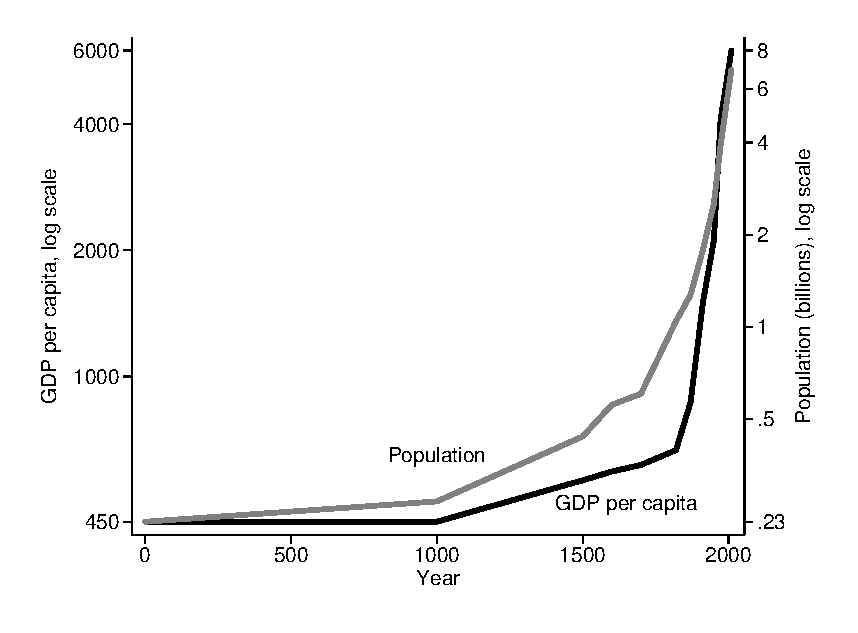
\includegraphics[scale=1.3]{figure_8_1.eps}
\end{center}
}

\slide{Eras}{
\begin{itemize}
	\item Malthusian Era (1 million BC to 1800-ish AD)
	\begin{itemize}
		\item Low population growth rates: 0.02-0.27\% per year
		\item Low $y$ growth rates: 0-0.14\% per year
	\end{itemize}
	\item Post-Malthusian Era (1800-ish AD to 1920-ish AD)
		\item Both population and $y$ accelerate
		\item Population growth rates: 0.4-1.0\% per year
		\item $y$ growth rates: 0.5-1.3\% per year
	\item Modern Growth Era (1920-ish AD to now)
	\begin{itemize}
		\item Continued $y$ growth, but Demographic Transition
		\item Population growth rates: falling below 0.5\% per year
		\item $y$ growth rates: approaching long-run trend of 1.85\% per year
	\end{itemize}
\end{itemize}
}

\slide{Malthusian Economy}{Production now includes a fixed factor, $X$
\begin{equation}
Y = B X^{\beta}L^{1-\beta}
\end{equation}
where $B$ is a measure of productivity. Output per worker is
\begin{equation}
y = B \left(\frac{X}{L}\right)^{\beta}
\end{equation}
Note that output per worker depends negatively on $L$ - this is the Malthusian effect

\vspace{.25in}\noindent Population growth is now endogenous - determined inside the model
\begin{equation}
\frac{\dot{L}}{L} = \theta(y - \underline{c})
\end{equation}
where $\underline{c}$ is the subsistence constraint. Below that, population falls as people do not consume enough (i.e. famine) while above $\underline{c}$ population rises. 
}

\slide{Malthusian Equilibrium}{Combine the two equations to get
\begin{equation}
\frac{\dot{L}}{L} = \theta\left(\left(\frac{X}{L}\right)^{\beta} - \underline{c}\right)
\end{equation}
\begin{center}
\scalebox{1.2}
{
\begin{pspicture}(10,9)
\psline{->}(0,3)(9,3) \psline{->}(0,0)(0,8) \rput(9.3,2.7){$L$} \rput(0,8.3){$\dot{L}/L$} 
\pscurve[linewidth=2pt](.5,8)(4,3)(8,1)(9,.9)
\psline[arrowsize=5pt 3]{->}(0,3)(.5,3) \psline[arrowsize=5pt 3]{->}(.5,3)(.9,3) \psline[arrowsize=5pt 3]{->}(.9,3)(1.3,3) \psline[arrowsize=5pt 3]{->}(1.3,3)(1.7,3)
\psline[arrowsize=5pt 3]{->}(1.7,3)(2.1,3) \psline[arrowsize=5pt 3]{->}(2.1,3)(2.5,3)
\psline[arrowsize=5pt 3]{->}(2.5,3)(2.9,3) \psline[arrowsize=5pt 3]{->}(2.9,3)(3.3,3)
\psline[arrowsize=5pt 3]{->}(3.3,3)(3.7,3)
\psline[arrowsize=5pt 3]{<-}(4.3,3)(4.7,3) \psline[arrowsize=5pt 3]{<-}(4.7,3)(5.1,3)
\psline[arrowsize=5pt 3]{<-}(5.1,3)(5.5,3) \psline[arrowsize=5pt 3]{<-}(5.5,3)(5.9,3)
\psline[arrowsize=5pt 3]{<-}(5.9,3)(6.3,3) \psline[arrowsize=5pt 3]{<-}(6.3,3)(6.7,3)
\psline[arrowsize=5pt 3]{<-}(6.7,3)(7.1,3) \psline[arrowsize=5pt 3]{<-}(7.1,3)(7.5,3)
\psline[arrowsize=5pt 3]{<-}(7.5,3)(7.9,3) \rput(-.3,3){$0$} \rput(4,2.7){$L^{\ast}$}
\rput(9.3,.4){$\frac{\dot{L}}{L} = \theta \left(B \left(\frac{X}{L}\right)^{\beta} - \underline{c} \right)$}
\end{pspicture}
}
\end{center}
}

\slide{Malthusian Equilibrium}{In steady state, we have that
\begin{equation}
L^{\ast} = \left( \frac{B}{\underline{c}}  \right)^{1/\beta} X
\end{equation}
and
\begin{equation}
y^{\ast} = \underline{c}.
\end{equation}

\vspace{.25in}\noindent Our model gives us a stagnant output per worker. Any productivity increase ($B$) gets translated into higher populations, not higher living standards. 

\vspace{.25in}\noindent $\underline{c}$ need not be bare miniumum subsistence, but it is the fixe output per worker in a Malthusian economy

}

\slide{Dismal Science}{Implications of the Malthusian model
\begin{itemize}
	\item Anything that kills lots of people ($L$ drops) will raise living standards
	\item Eventually people will breed themselves back to lower living standards
\end{itemize}

\vspace{.25in}\noindent Black Death in Europe, 14th-15th century
\begin{itemize}
	\item England: population falls from 3.75 million to 2 million, real wage doubles
	\item Italy: population falls from 10 million to 7 million, real wage up by 2.5 times
\end{itemize}
By 1500 both had wages back to pre-Black Death levels, and populations back at prior levels

}

\slide{Technological Change}{A one-off shift up in $B$ raises steady-state population
\begin{center}
\scalebox{1.2}
{
\begin{pspicture}(10,9)
\psline{->}(0,3)(9,3) \psline{->}(0,0)(0,8) \rput(9.3,2.7){$L$} \rput(0,8.3){$\dot{L}/L$} 
\pscurve[linewidth=2pt](.5,8)(4,3)(8,1)(9,.9) \psline{->}(1.5,7)(2.7,7) \rput(2,7.3){$B \uparrow$}
\pscurve[linewidth=2pt,linecolor=gray](2.5,8)(6,3)(10,1)(11,.9) \rput(-.3,3){$0$} \rput(4,2.5){$L_1^{\ast}$} \rput(6,2.5){$L_2^{\ast}$} \psdot(4,5.5) \psdot(4,3) \psdot(6,3) \rput(4.1,5.8){$A$}
\psline[arrowsize=5pt 3]{->}(4.3,3)(4.7,3) \psline[arrowsize=5pt 3]{->}(4.7,3)(5.1,3)
\psline[arrowsize=5pt 3]{->}(5.1,3)(5.5,3) \psline[arrowsize=5pt 3]{->}(5.5,3)(5.9,3)
\rput(9.3,.4){$\frac{\dot{L}}{L} = \theta \left(B \left(\frac{X}{L}\right)^{\beta} - \underline{c} \right)$}
\end{pspicture}
}
\end{center} 
}

\slide{Continuous Technological Change}{Take the logs and derivative of production function
\begin{equation}
y = B \left(\frac{X}{L}\right)^{\beta}
\end{equation}
to get
\begin{equation}
\frac{\dot{y}}{y} = \frac{\dot{B}}{B} - \frac{1}{\beta}\frac{\dot{L}}{L}
\end{equation}
and let $g = 1/\beta \dot{B}/B$ for convenience.

\vspace{.25in}\noindent Then
\begin{itemize}
	\item If $\dot{L}/L > g$, output per worker is rising
	\item If $\dot{L}/L < g$, output per worker is falling
	\item If $\dot{L/L} = g$, output per worker is constant
\end{itemize}
}

\slide{With Population Growth}{Combine this with 
\begin{equation}
\frac{\dot{L}}{L} = \theta(y - \underline{c})
\end{equation}
\begin{center}
\scalebox{1.2}
{
\begin{pspicture}(10,9)
\psline{->}(0,0)(9,0) \psline{->}(0,0)(0,8) \rput(9.3,-.3){$y$} \rput(0,8.3){$\dot{L}/L$} 
\psline[linewidth=2pt](0,0)(6,8.4) \psline[linewidth=2pt,linecolor=gray](0,2.8)(9,2.8)
\psline[linestyle=dashed,dash=3pt 2pt](2,0)(2,2.8) \rput(2,-.4){$y^M$} \rput(-.6,2.8){$g$}
\psline[arrowsize=5pt 3]{->}(0,0)(.5,0) \psline[arrowsize=5pt 3]{->}(.5,0)(.9,0) \psline[arrowsize=5pt 3]{->}(.9,0)(1.3,0) \psline[arrowsize=5pt 3]{->}(1.3,0)(1.7,0)
\psline[arrowsize=5pt 3]{<-}(2.3,0)(2.7,0) \psline[arrowsize=5pt 3]{<-}(2.7,0)(3.1,0)
\psline[arrowsize=5pt 3]{<-}(3.1,0)(3.5,0) \psline[arrowsize=5pt 3]{<-}(3.5,0)(3.9,0)
\psline[arrowsize=5pt 3]{<-}(3.9,0)(4.3,0) \psline[arrowsize=5pt 3]{<-}(4.3,0)(4.7,0)
\psline[arrowsize=5pt 3]{<-}(4.7,0)(5.1,0) \psline[arrowsize=5pt 3]{<-}(5.1,0)(5.5,0)
\psline[arrowsize=5pt 3]{<-}(5.5,0)(5.9,0)
\rput(6,6){$\frac{\dot{L}}{L} = \theta \left(y - \underline{c} \right)$}
\end{pspicture}
}
\end{center}
}

\slide{Endogenous Technology}{With constant technological progress at $g$
\begin{itemize}
	\item Population size grows continuously (matching Malthusian era data)
	\item Steady state output per worker is stagnant (matching Malthusian era data)
\end{itemize}

\vspace{.25in}\noindent We match history better. But where does $g$ come from? We can introduce endogenous technological progress
\begin{equation}
\frac{\dot{B}}{B} = \nu \frac{s_R L^{\lambda}}{B^{1-\phi}}
\end{equation}
which is just like our endogenous model from before. But focus on non-steady state behavior.

\vspace{.25in}\noindent If $L$ is very small compared to $B$, then as $L$ goes up, $\dot{B}/B$ goes up. So the more people, the faster is technological progress. Scale effects.
}

\slide{Kremer Model}{Simplify endogenous technology by setting $\lambda=1$ and $\phi=1$. (We said $\phi=1$ is wrong, generally, but will work for the period of time when $L$ was very low). Assume $s_R = 1$ for simplicity.
\begin{equation}
\frac{\dot{B}}{B} = \nu L
\end{equation}
and combine with the steady state condition that $\dot{L}/L = g = 1/\beta (\dot{B}/B)$ gives us
\begin{equation}
\frac{\dot{L}}{L} = \frac{\nu}{\beta}L
\end{equation}

\vspace{.25in}\noindent Implication is that the growth rate of popuation (which depends on technological growth) is positively related to the \textit{size} of the population (which drives technological growth).

}

\slide{Population Growth Over Very Long-Run}{
\begin{center}
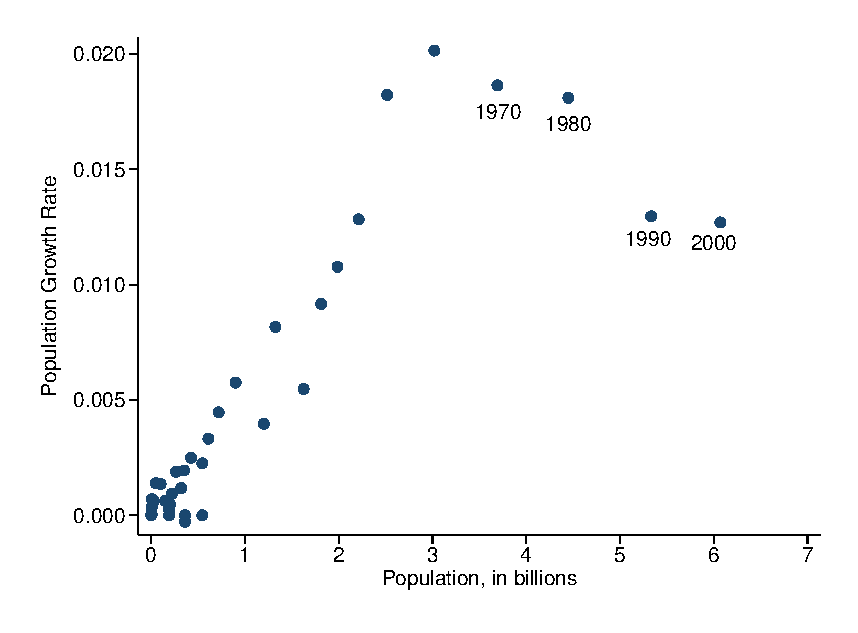
\includegraphics[scale=1.3]{figure_8_5.eps}
\end{center}
}

\slide{Transition to Modern Growth}{Kremer model works for most of history.
\begin{itemize}
	\item Breaks down in 20th century
	\item Population growth has not spiraled up continuously
	\item Rate of technological change has not spiraled up continuously
\end{itemize}

\vspace{.25in}\noindent We need to adapt the model to capture the endogenous response to population to higher output per worker (Demographic Transition) that ensures world ends up with constant technological change (as in the Romer/Schumpeter models).

}

\slide{More Realistic Population Growth Function}{Rather than linear $\frac{\dot{L}}{L} = \theta(y - \underline{c})$, let population growth look like this:
\begin{center}
\scalebox{1.2}
{
\begin{pspicture}(10,9)
\psline{->}(0,0)(9,0) \psline{->}(0,0)(0,8) \rput(9.3,-.3){$y$} \rput(0,8.3){$\dot{L}/L$} 
\pscurve[linewidth=2pt](0,0)(4,5)(7,2)(9,1.8) \psline[linewidth=2pt,linecolor=gray](0,2.8)(9,2.8)
\psline[linestyle=dashed,dash=3pt 2pt](1.48,0)(1.48,2.8) \psline[linestyle=dashed,dash=3pt 2pt](6.1,0)(6.1,2.8) \rput(1.48,-.4){$y^M$} \rput(6.1,-.4){$y^T$} \rput(-.6,2.8){$g$}
\psline[arrowsize=5pt 3]{->}(0,0)(.5,0) \psline[arrowsize=5pt 3]{->}(.5,0)(.9,0) \psline[arrowsize=5pt 3]{->}(.9,0)(1.3,0)
\psline[arrowsize=5pt 3]{<-}(1.5,0)(1.9,0) \psline[arrowsize=5pt 3]{<-}(1.9,0)(2.3,0)
\psline[arrowsize=5pt 3]{<-}(2.3,0)(2.7,0) \psline[arrowsize=5pt 3]{<-}(2.7,0)(3.1,0)
\psline[arrowsize=5pt 3]{<-}(3.1,0)(3.5,0) \psline[arrowsize=5pt 3]{<-}(3.5,0)(3.9,0)
\psline[arrowsize=5pt 3]{<-}(3.9,0)(4.3,0) \psline[arrowsize=5pt 3]{<-}(4.3,0)(4.7,0)
\psline[arrowsize=5pt 3]{<-}(4.7,0)(5.1,0) \psline[arrowsize=5pt 3]{<-}(5.1,0)(5.5,0)
\psline[arrowsize=5pt 3]{<-}(5.5,0)(5.9,0) \psline[arrowsize=5pt 3]{->}(6.2,0)(6.6,0)
\psline[arrowsize=5pt 3]{->}(6.6,0)(7.0,0) \psline[arrowsize=5pt 3]{->}(7.0,0)(7.4,0)
\psline[arrowsize=5pt 3]{->}(7.4,0)(7.8,0) \psline[arrowsize=5pt 3]{->}(7.8,0)(8.2,0)
\rput(6,5.5){Population growth function}
\end{pspicture}
}
\end{center}
}

\slide{From Malthusian Stagnation to Modern Growth}{The transition is driven by the interplay of population size and technological change
\begin{itemize}
	\item Malthusian era:
	\begin{itemize}
		\item Population, $L$, is small, so technological growth, $g$, is low
		\item Low $g$ means low $y^M$, Malthusian steady state income
	\end{itemize}
	\item Post-Malthusian era:
	\begin{itemize}
		\item Population, $L$, reaches a sufficiently large size that $g$ gets big (above max of population growth function)
		\item This accelerates population growth $\dot{L}/L$ while also allowing $y$ to rise continuously
	\end{itemize}
	\item Modern Growth era:
	\begin{itemize}
		\item Population, $L$, is still very large, but $B$ has risen so much that $g$ slows down
		\item Population growth, $\dot{L}/L$, slows down as economy gets richer
		\item Eventually population growth levels off at some constant, where we are in Romer/Schumpeter model
	\end{itemize}
\end{itemize}

}

\slide{Growth in Modern Growth Regime}{Slightly different answer for long-run growth than Romer/Schumpeter.
We know that steady state technology growth is
\begin{equation}
\frac{\dot{B}}{B} = \frac{\lambda}{1-\phi}n^{\ast}
\end{equation}
where $n^{\ast}$ is the long-run population growth rate.

\vspace{.25in}\noindent But growth in output per worker is
\begin{eqnarray}
\frac{\dot{y}}{y} &=& \frac{\dot{B}}{B} - \frac{1}{\beta}\frac{\dot{L}}{L} \\
                  &=& \frac{\lambda}{1-\phi}n^{\ast} - \frac{1}{\beta}n^{\ast} \\
				  &=& \left(\frac{\lambda}{1-\phi} - \frac{1}{\beta}\right)n^{\ast}
\end{eqnarray}
There is this additional ``drag'' on economic growth of $1/\beta$ which captures the influence of the fixed factor of production, $X$. So long as $\lambda/(1-\phi)$ is large enough, innovation outweights Malthusian effects of fixed resource.

}

\slide{Structural Change}{Reason that innovation tends to win is that as we get richer, $\beta$ falls. That is, fixed resources (land, energy) become less important in production. We'll revisit this in another chapter. 
\begin{center}
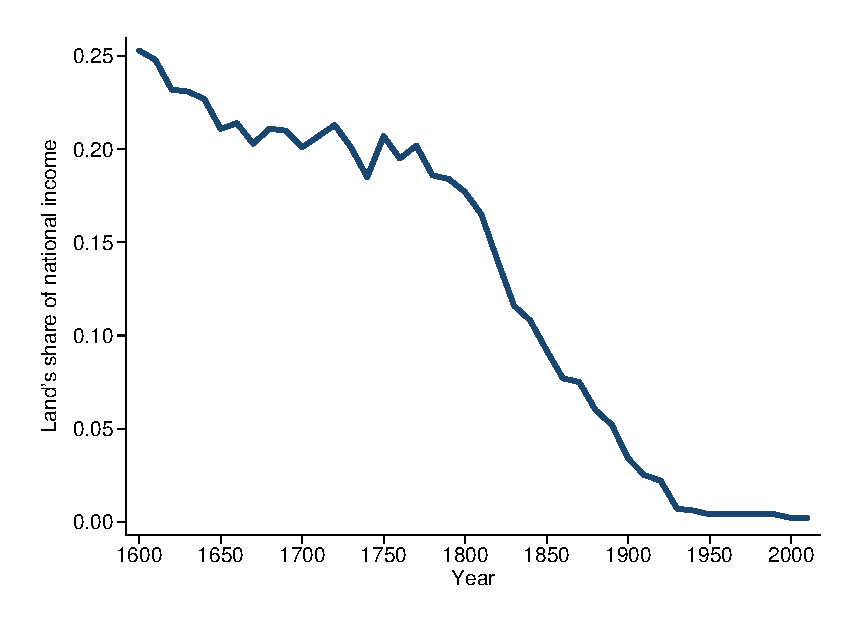
\includegraphics[scale=1.2]{figure_8_8.eps}
\end{center}

}

\slide{Economic of Population Growth}{Model of quality/quantity trade-off
\begin{equation}
y = \underline{c} + M + E
\end{equation}
\begin{itemize}
	\item $\underline{c}$ is consumption of output
	\item $M$ is amount spent having kids (their food, their clothes)
	\item $E$ is amount spent on kid ``quality'' (education, violin lessons, etc..)
\end{itemize}

\vspace{.25in}\noindent Spending translates into kids ($m$) and education level ($u$) as
\begin{eqnarray}
m &=& \eta \frac{M}{y} \\ 
u &=& E + \overline{u}
\end{eqnarray}
where $m$ depends negatively on income (opportunity cost of time for parents). $u$ has a fixed component $\overline{u}$ that kids get for ``free''.
}

\slide{Utility and Optimization}{Families have a utility function of
\begin{equation}
V = \ln{m} + \ln{u}
\end{equation}
and to solve for optimal choices of $m$ and $u$, first put in terms of spending
\begin{equation}
V = \ln\left(\eta \frac{M}{y}\right) + \ln\left(E+\overline{u}\right)
\end{equation}
and then use budget constraint to put in terms of only $E$
\begin{equation}
V = \ln\left(\eta \frac{y-\underline{c}-E}{y}\right) + \ln\left(E+\overline{u}\right)
\end{equation} 

\vspace{.25in}\noindent First-order condition with respect to $E$ is
\begin{equation}
\frac{-1}{y-\underline{c}-E} + \frac{1}{E+ \overline{u}} = 0
\end{equation}

}

\slide{Optimal Education}{With FOC
\begin{equation}
\frac{-1}{y-\underline{c}-E} + \frac{1}{E+ \overline{u}} = 0
\end{equation}
solving to
\begin{equation}
E = \frac{y-\overline{u} - \underline{c}}{2}
\end{equation}
we've got optimal spending on kids. But note that $E$ could go below zero, which isn't possible.

\vspace{.25in}\noindent Need to account for corner solution where $E=0$. Means we have
\begin{center}
\begin{tabular}{ll}
$E = 0$ & if $y < \underline{c} + \overline{u}$ \\ \\
$E = \frac{y-\overline{u} - \underline{c}}{2}$ & if $y \geq \underline{c} + \overline{u}$ \\
\end{tabular}
\end{center}

\vspace{.25in}\noindent Important implications are that $E = 0$ when families are poor, but $E>0$ when families get over a certain income level.
}

\slide{Optimal Fertility}{Using optimal $E$ answer, solve for $m$
\begin{center}
\begin{tabular}{ll}
$m = \eta \left(1 - \frac{\underline{c}}{y} \right)$ & if $y < \underline{c} + \overline{u}$ \\ \\
$m = \frac{\eta}{2}\left(1 - \frac{\underline{c}}{y} + \frac{\overline{u}}{y}  \right)$ & if $y \geq \underline{c} + \overline{u}$ \\
\end{tabular}
\end{center}

\vspace{.25in}\noindent Important implications:
\begin{itemize}
	\item For sufficiently low income, $m$ is increasing with $y$ ($\partial m/\partial y >0$)
	\item Once income is $y \geq \underline{c} + \overline{u}$ then $m$ is decreasing with $y$ ($\partial m/\partial y < 0$)
\end{itemize}
Gives us the hill-shaped relationship of population growth and income per capita we used to model transition. 
}

\slide{Quality/Quantity}{What is happening
\begin{itemize}
	\item At low levels of income, all children get $\overline{u}$ for free. Marginal utility is higher in having another kid than in education existing ones to more than $\overline{u}$. 
	\item At higher levels of income, parents want kids with $u > \overline{u}$, so they have to spend on this. This leaves less for having greater numbers of kids (as each needs to get $u$ education).
	\item As incomes get high enough, parents trade quantity for quality - the Demographic Transition
\end{itemize}

\vspace{.25in}\noindent This prevents the Malthusian world from continuing on indefinitely. Eventually population growth just doesn't keep up with technological progress. 
\begin{itemize}
	\item But greater population continues to propel technological change
	\item That technological change gets used to raise $y$ as opposed to $L$ by parents who value education/quality
\end{itemize}
}

\end{document}